\documentclass[a4paper, 12pt]{article}%тип документа

%отступы
\usepackage[left=1.5cm,right=1cm,top=2cm,bottom=3cm,bindingoffset=0cm]{geometry}
\setlength{\parindent}{5ex}

%Русский язык
\usepackage[T2A]{fontenc} %кодировка
\usepackage[utf8]{inputenc} %кодировка исходного кода
\usepackage[english,russian]{babel} %локализация и переносы

%Вставка картинок
\usepackage{graphicx}
\graphicspath{{pictures/}}
\DeclareGraphicsExtensions{.pdf,.png,.jpg,}
\usepackage{wrapfig}

%Графики
\usepackage{pgfplots}
\pgfplotsset{compat=1.9}

%Математика
\usepackage{amsmath, amsfonts, amssymb, amsthm, mathtools}

%Таблицы
\usepackage{longtable} 
\usepackage{float}

%Римские цифры
\newcommand{\RomanNumeralCaps}[1]{\uppercase\expandafter{\romannumeral#1}}

\usepackage{multirow}



\begin{document}
	\begin{titlepage}
		\begin{center}
			\textsc{Федеральное государственное автономное образовательное учреждение высшего образования«Московский физико-технический институт (национальный исследовательский университет)»\\[5mm]
			}
			
			\vfill
			
			\textbf{Отчёт по лабораторной работе 5.4.2\\[3mm]
				Исследование энергетического спектра $\beta$-частиц
				и определение их максимальной энергии при помощи
				магнитного спектрометра
				\\[50mm]
			}
			
		\end{center}
		
		\hfill
		\begin{minipage}{.5\textwidth}
			Выполнил студент:\\[2mm]
			Сериков Василий Романович\\[2mm]
			группа: Б03-102\\[5mm]
			
		\end{minipage}
		\vfill
		\begin{center}
			Москва, 2023 г.
		\end{center}
		
	\end{titlepage}
	
	\newpage
	\setcounter{page}{2}
	\textbf{Аннотация}\\
	
	\textbf{Цель работы: }\\
	
	 С помощью магнитного спектрометра исследовать энергетический спектр $\beta$ - частиц при распаде ядер $^{137}$Cs  и определить их максимальную энергию.\\ 
	
	\textbf{Теоретическое введение: }\\
	
	Бета-распадом называется самопроизвольное превращение ядер, при котором их массовое число не изменяется, а заряд увеличивается или уменьшается на единицу. Бета-активные ядра встречаются во всей области значений массового числа A, начиная от единицы (свободный нейтрон) и кончая самыми тяжелыми ядрами. Период полураспада $\beta$ - активных ядер изменяется от ничтожных долей секунды до $10^{18}$ лет. Выделяющаяся при единичном акте $\beta$ - распада энергия варьируется от 18 кэВ до 13,4 МэВ.
	
	В данной работе мы будем иметь дело с электронным распадом
	
	\begin{equation}\label{}
		^A_ZX \rightarrow ^{\; \; \; \; \: A}_{Z+1}X + e^- + \widetilde{\nu}
	\end{equation}
	
	при котором кроме электрона испускается антинейтрино. Освобождающаяся при $\beta$-распаде энергия делится между электроном, антинейтрино и дочерним ядром, однако доля энергии, передаваемой ядру, исчезающе мала по сравнению с энергией, уносимой электроном и антинейтрино. Практически можно считать, что эти две частицы делят между собой всю освобождающуюся энергию. Поэтому электроны могут иметь любое значение энергии  от нулевой до некоторой максимальной, которая равна энергии, освобождающейся при $\beta$-распаде, являющейся важной физической величиной.
	
	Вероятность $ dw $ того, что при распаде электрон вылетит с импульсом в интервале $d^3p$, а антинейтрино с импульсом в интервале $d^3k$, пропорциональна произведению этих дифференциалов. Но мы должны еще учесть закон сохранения энергии, согласно которому импульсы $ p $ и $ k $ электрона и антинейтрино связаны соотношением
	
	\begin{equation}
		E_e - E - ck = 0,
	\end{equation}
	
	где $E_e$ - максимальная энергия электрона, кинетическая энергия электрона $ E $ связана с его импульсом обычным релятивистским соотношением
	
	\begin{equation}
		E = c\sqrt{p^2 + m^2c^2} - mc^2,
	\end{equation}
	
	а через $ ck $ обозначена энергия антинейтрино с импульсом $ k $. Условие можно учесть введением в выражение для $ dw $ $\delta$ - функции
	\begin{equation}
		\delta (E_e - E - ck).
	\end{equation}
	
	Таким образом, вероятность $ dw $ может быть записана в виде
	
	\begin{equation}\label{dw}
		dw = D \delta (E_e - E - ck)d^3 p d^3 k = D \delta (E_e - E - ck)p^2dpk^2dkd{\Omega}_ed{\Omega}_{\widetilde{\nu}},
	\end{equation}
	
	где $ D $ --- некоторый коэффициент пропорциональности, $d\Omega_e$ , $d\Omega_{\widetilde{\nu}}$ --- элементы телесных углов направлений вылета электрона и нейтрино. Вероятность $ dw $ непосредственно связана с $\beta$-спектром, поскольку для большого числа $N_0$ распадов число $dN$ распадов с вылетом электрона и антинейтрино с импульсом соответственно от $ p $ до $ p + dp $ и от
	$ k $ до $ k + d $k определяется соотношением
	
	\begin{equation}\label{dn = n_0 dw}
		dN = N_0 dw  
	\end{equation}
	
	Коэффициент $ D $ в формуле \eqref{dw} можно считать для рассматриваемых нами так называемых разрешенных фермиевских типов распадов с хорошей точностью константой (разрешенными называются такие переходы, при которых не изменяются ни момент, ни четность состояния ядра). В этом случае величину $ dw $ из \eqref{dn = n_0 dw} можно проинтегрировать по всем углам и по абсолютному значению импульса нейтрино.
	
	После умножения на полное число распадов $ N $ проинтегрированное выражение приобретает смысл числа электронов $ dN $, вылетающих из ядра с импульсом, абсолютная величина которого лежит между $ p $ и$  p + dp $:
	
	\begin{equation}\label{dN}
		dN = \dfrac{16\pi^2 N_0}{c^2}Dp^2(E_e - E)^2dp.
	\end{equation}
	
	Чтобы получить распределение электронов по энергиям, надо в \eqref{dN} перейти от $ dp $ к $ dE $:
	
	\begin{equation}
		dE = \dfrac{c^2p}{E + mc^2}dp,
	\end{equation}
	
	после чего выражающая форму $\beta$ --- спектра величина $ N(E) = dN/dE $
	приобретает вид
	
	\begin{equation}\label{dN/dE big}
		\dfrac{dN}{dE} = N_0Bcp(E + mc^2)(E_e - E)^2 = N_0B\sqrt{E(E + 2mc^2)}(E_e - E)^2(E + mc^2)
	\end{equation}
	
	где $B = (16\pi^2/c^4)D$. В нерелятивистском приближении, которое и имеет место с нашем случае, выражение \eqref{dN/dE big} упрощается, и мы имеем
	
	\begin{equation}\label{dN/dE}
		\dfrac{dN}{dE} \approx \sqrt{E}(E_e - E)^2.
	\end{equation}
	
	\begin{figure}[H]
		\centering
		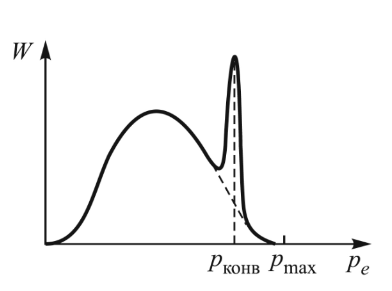
\includegraphics[width=0.5\linewidth]{spectr}
		\caption{Форма спектра $\beta$-частиц
			при разрешенных переходах}
	\end{figure}
	
	
	Выражение \eqref{dN/dE} приводит к спектру, имеющему вид широкого колокола (рис 1). Кривая плавно отходит от нуля и столь же плавно, по параболе, касается оси абсцисс в области максимальной энергии электронов $E_e$. 
	
	Дочерние ядра, возникающие в результате $\beta$-распада, нередко оказываются возбужденными. Возбужденные ядра отдают свою энергию либо излучая $\gamma$-квант (энергия которого равна разности энергий начального и конечного уровней), либо передавая избыток энергии одному из электронов с внутренних оболочек атома. Излучаемые в таком процессе электроны имеют строго определенную энергию и называются конверсионными.
	
	Конверсия чаще всего происходит на оболочках $ K $ или $ L $. На спектре, представленном на рис. \ref{ris spetr}, видна монохроматическая линия, вызванная электронами конверсии. Ширина этой линии в нашем случае является чисто аппаратурной, по ней можно оценить разрешающую силу спектрометра.
	
	
	\section{Экспериментальная установка}
	
	Для определения энергии $\beta$-частиц в работе используется магнитный спектрометр, схема которого показана на рисунке \ref{pic:scheme} слева. Электроны испускаются радиоактивным источником и попадают в магнитное поле катушки, ось которой параллельна $OZ$. Траектории электронов сходятся в одной точке --- фокусе, где и установлен сцинтилляционный счетчик, сигналы которого усиливаются фотоумножителем и регистрируются пересчетным прибором. Фокусное расстояние $f$ магнитной линзы связано с током в катушке $I$ и импульсом $p_e$ регистрируемых частиц следующим образом:
	
	\[ \frac{1}{f} \propto \frac{I^2}{p_e^2} \]  
	
	При неизменной геометрии установки, увеличивая и уменьшая силу тока, можно фокусировать электроны разных импульсов, причем 
	
	\begin{equation}\label{k}
		p_e = kI,
	\end{equation}
	
	где $k$ --- коэффициент пропорциональности, являющийся параметром установки.
	
	\begin{figure}[h]
		\centering
		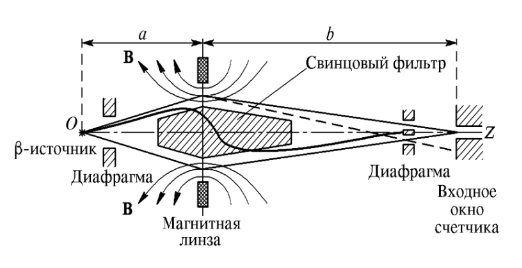
\includegraphics[width=0.48\textwidth]{lab}
		\hfill
		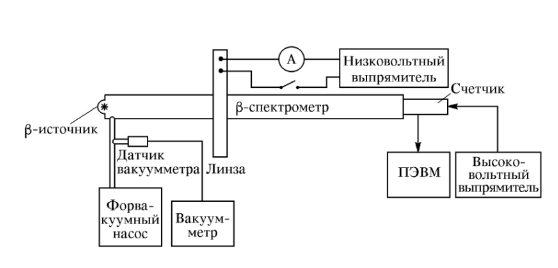
\includegraphics[width=0.48\textwidth]{lab2}
		\caption{слева --- схема $\beta$-спектрометра; справа --- блок-схема установки для изучения спектра}
		\label{pic:scheme}
	\end{figure}
	
	В $\beta$-спектрометре установлены диафрагмы для ограничения углов вылета частиц из источника и свинцовый фильтр для защиты от прямого попадания $\gamma$-лучей. 
	
	Число частиц $N$, регистрируемых на установке, равно: $N \approx W \cdot \Delta p_e$, где $\Delta p_e$ - разрешающая способность спектрометра. Дифференцируя выражение для форуса магнитной линзы, получим: $\Delta p_e = \frac{1}{2}\frac{\Delta f}{f}p_e$, то есть $\Delta p_e \propto p_e$. Таким образом, для количества частиц справедлива формула: 
	
	\begin{equation}\label{N}
		N = CW(p_e)p_e 
	\end{equation}
	
	Здесь $C$ - некоторая константа.\\
	
	
	\textbf{Ход работы: }\\
	
	\begin{enumerate}
		
		
		\item  Перед проведением измерения $\beta$-спектра, проведем измерения фона. Полученные результаты занесем в таблицу 1.
		
		\begin{longtable}{|c|c|c|c|c|c|}
			\hline
			№ & 1 & 2 & 3 & 4 & 5\\ \hline
			$N_{\text{фон}}$ & 1,068 & 1,134 & 1,085 & 1,102 & 0,908 \\ \hline
			$dN_{\text{фон}}$ & 0,086 & 0,097 & 0,087 & 0,074 & 0,055 \\ \hline
			\caption{Число срабатываний счетчика в секунду при измерении фона t = 100 сек}
		\end{longtable}
		
		
		Посчитаем среднее значение $\overline{n_{\text{фон}}}$ числа срабатываний счетчика 
			
		
		$$\overline{N_{\text{фон}}} = \frac{1}{5} \sum_{i = 1}^{5} n_i = 1,05 \pm 0,07$$
		
		\item Проведем серию измерений $\beta$-спектра, изменяя ток магнитной линзы в интервале 0А -- 5А. Прокалибруем спектрометр с учетом, что величина произведения импульса конверсионного электрона на скорость света равна 1013,5 кэВ. Полученные данные занесем в таблицу 2.
		
		\begin{longtable}{|c|c|c|c|c|c|}
			\hline
			№   & I, А  & N      & p, кэВ/с  & T, кэВ  & $\sqrt{(N(p) - \overline{N_{\text{фон}}})}/p^{3/2} \cdot 10^6)$   \\ \hline
			1   & 0,2   & 0,977  & 51,9      & 2,6     & 0     \\ \hline
			2   & 0,4   & 0,889  & 98,8      & 9,5     & 0     \\ \hline
			3   & 0,6   & 0.900  & 148,2     & 21,1    & 0     \\ \hline
			4   & 0,8   & 1,488  & 197,6     & 36,9    & 179,9 \\ \hline
			5   & 1,0   & 1,711  & 247,0     & 56,6    & 165,1 \\ \hline
			6   & 1,2   & 2,288  & 296,5     & 79,8    & 176,4 \\ \hline
			7   & 1,4   & 3,143  & 345,9     & 106,0   & 186,3 \\ \hline
			8   & 1,6   & 3,699  & 395,3     & 135,0   & 175,1 \\ \hline
			9   & 1,8   & 4,075  & 444,7     & 166,4   & 159,7 \\ \hline
			10  & 2,0   & 4,161  & 494,1     & 199,8   & 150,4 \\ \hline
			11  & 2,1   & 4,261  & 518,8     & 217,2   & 142,5 \\ \hline
			12  & 2,2   & 4,711  & 543,5     & 235,0   & 142,2 \\ \hline
			13  & 2,3   & 4,311  & 568,3     & 253,2   & 126,0 \\ \hline
			14  & 2,4   & 4,023  & 592,9     & 271,7   & 106,8 \\ \hline
			15  & 2,6   & 3,574  & 642,3     & 309,8   & 88,1  \\ \hline
			16  & 2,8   & 3,074  & 691,7     & 349,0   & 71,0  \\ \hline
			17  & 3,0   & 2,624  & 743,6     & 391,3   & 57,3  \\ \hline
			18  & 3,2   & 1,762  & 790,5     & 430,3   & 35,8  \\ \hline
			19  & 3,4   & 1,474  & 840,0     & 472,2   & 27,1  \\ \hline
			20  & 3,5   & 1,287  & 864,7     & 493,4   & 20,2  \\ \hline
			21  & 3,6   & 1,100  & 889,4     & 514,7   & 11,4  \\ \hline
			22  & 3,7   & 1,737  & 914,1     & 536,2   & 29,5  \\ \hline
			23  & 3,8   & 3,474  & 938,8     & 557,8   & 52,6  \\ \hline
			24  & 3,9   & 4,511  & 963,5     & 579,6   & 60,3  \\ \hline
			25  & 4,0   & 5,460  & 988,2     & 601,5   & 66,7  \\ \hline
			26  & 4,05  & 5,420  & 1000,5    & 612,5   & 70,9  \\ \hline
			27  & 4,1   & 6,235  & 1012,9    & 623,5   & 62,4  \\ \hline
			28  & 4,15  & 5,198  & 1025,2    & 634,5   & 60,0  \\ \hline
			29  & 4,2   & 5,023  & 1037,6    & 645,6   & 49,6  \\ \hline
			30  & 4,3   & 3,961  & 1062,3    & 667,8   & 27,3  \\ \hline
			31  & 4,4   & 1,962  & 1087,0    & 690,1   & 0     \\ \hline
			32  & 4,5   & 0,850  & 1111,7    & 712,5   & 0     \\ \hline
			33  & 4,6   & 0,625  & 1136,4    & 735,0   & 0     \\ \hline
			34  & 4,8   & 0,475  & 1185,8    & 780,2   & 0     \\ \hline
			35  & 5,0   & 0,275  & 1235,2    & 825,7   & 0     \\ \hline
			
			\caption{Данные с ЭВМ по результатам измерения количества частиц, импульса, энергии и коэффициентов Ферми-Кюри при различных значениях тока накала. Расчет p, T, коэффициентов Ферми-Кюри проводился с учетом фона.}
		\end{longtable}
		
		\item По полученным данным построим графики зависимости $N(p)$, $N(I)$ и график Ферми-Кюри.
		
		
		\begin{figure}[H]
			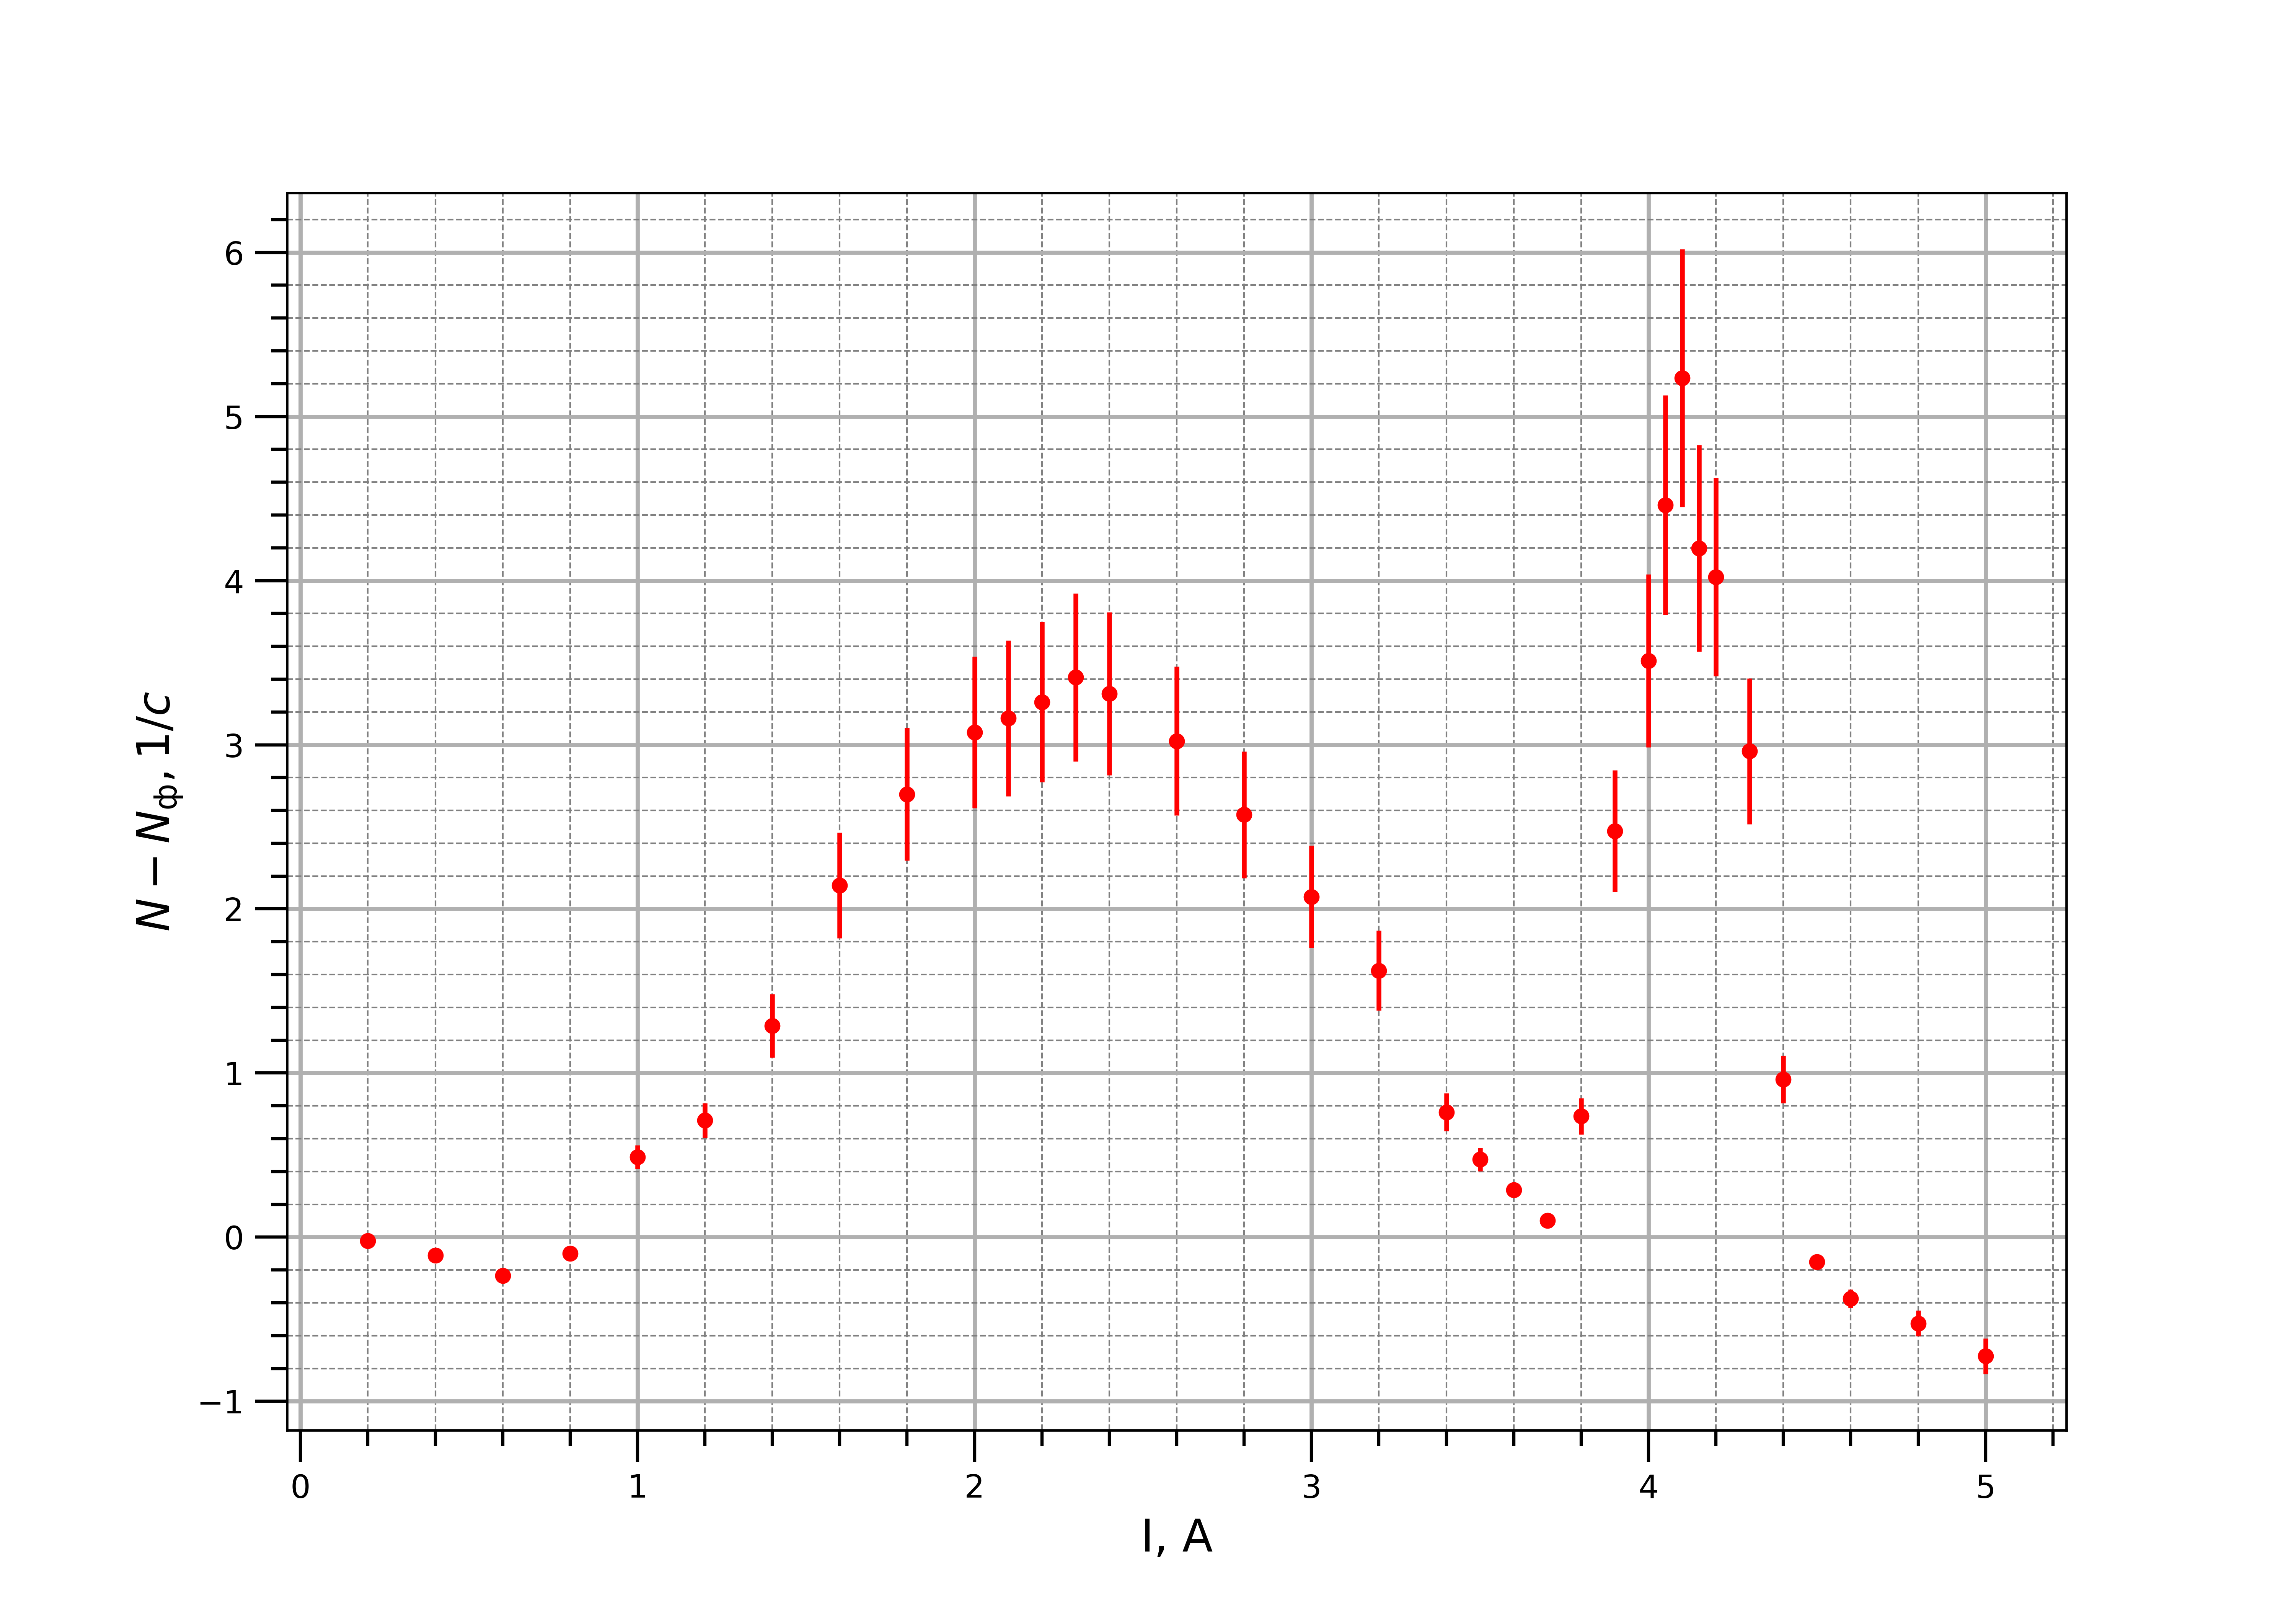
\includegraphics[scale=0.8]{N(I)}
			\centering
			\caption{График зависимости $N(I)$}
		\end{figure}
		
		\begin{figure}[H]
			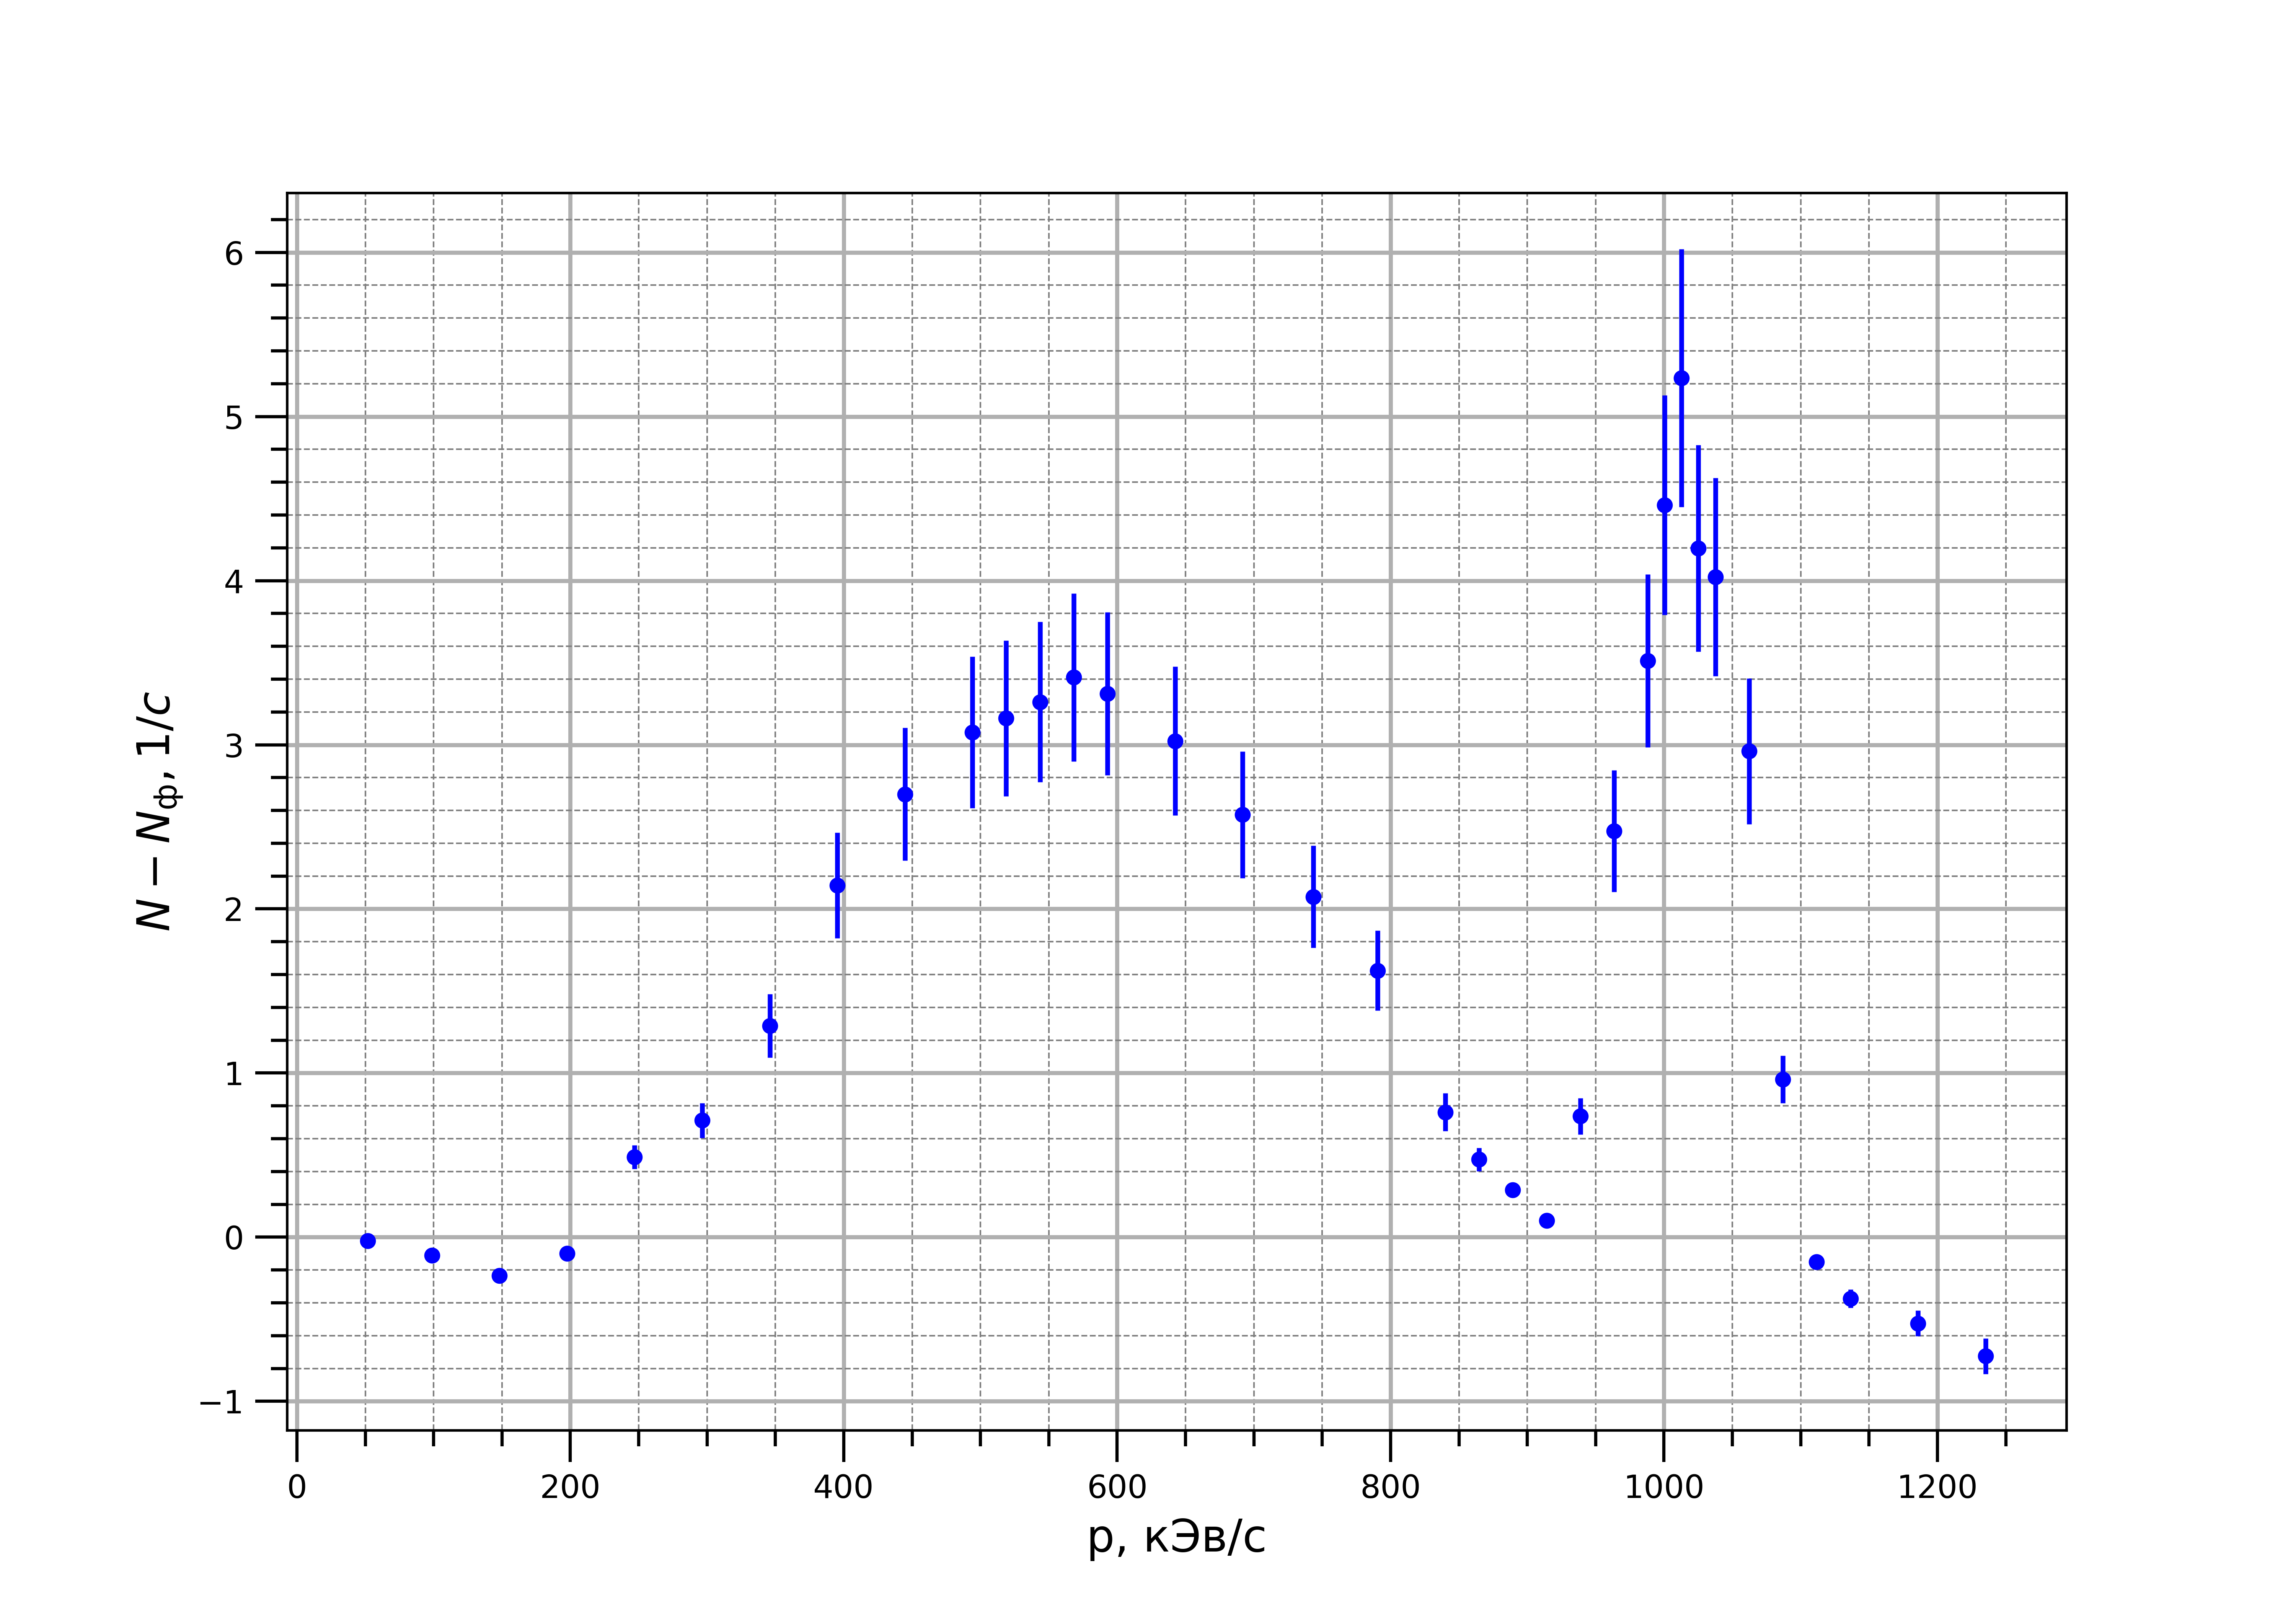
\includegraphics[scale=0.8]{N(p)}
			\centering
			\caption{График зависимости $N(p)$}
		\end{figure}
		
		
		\begin{figure}[H]
			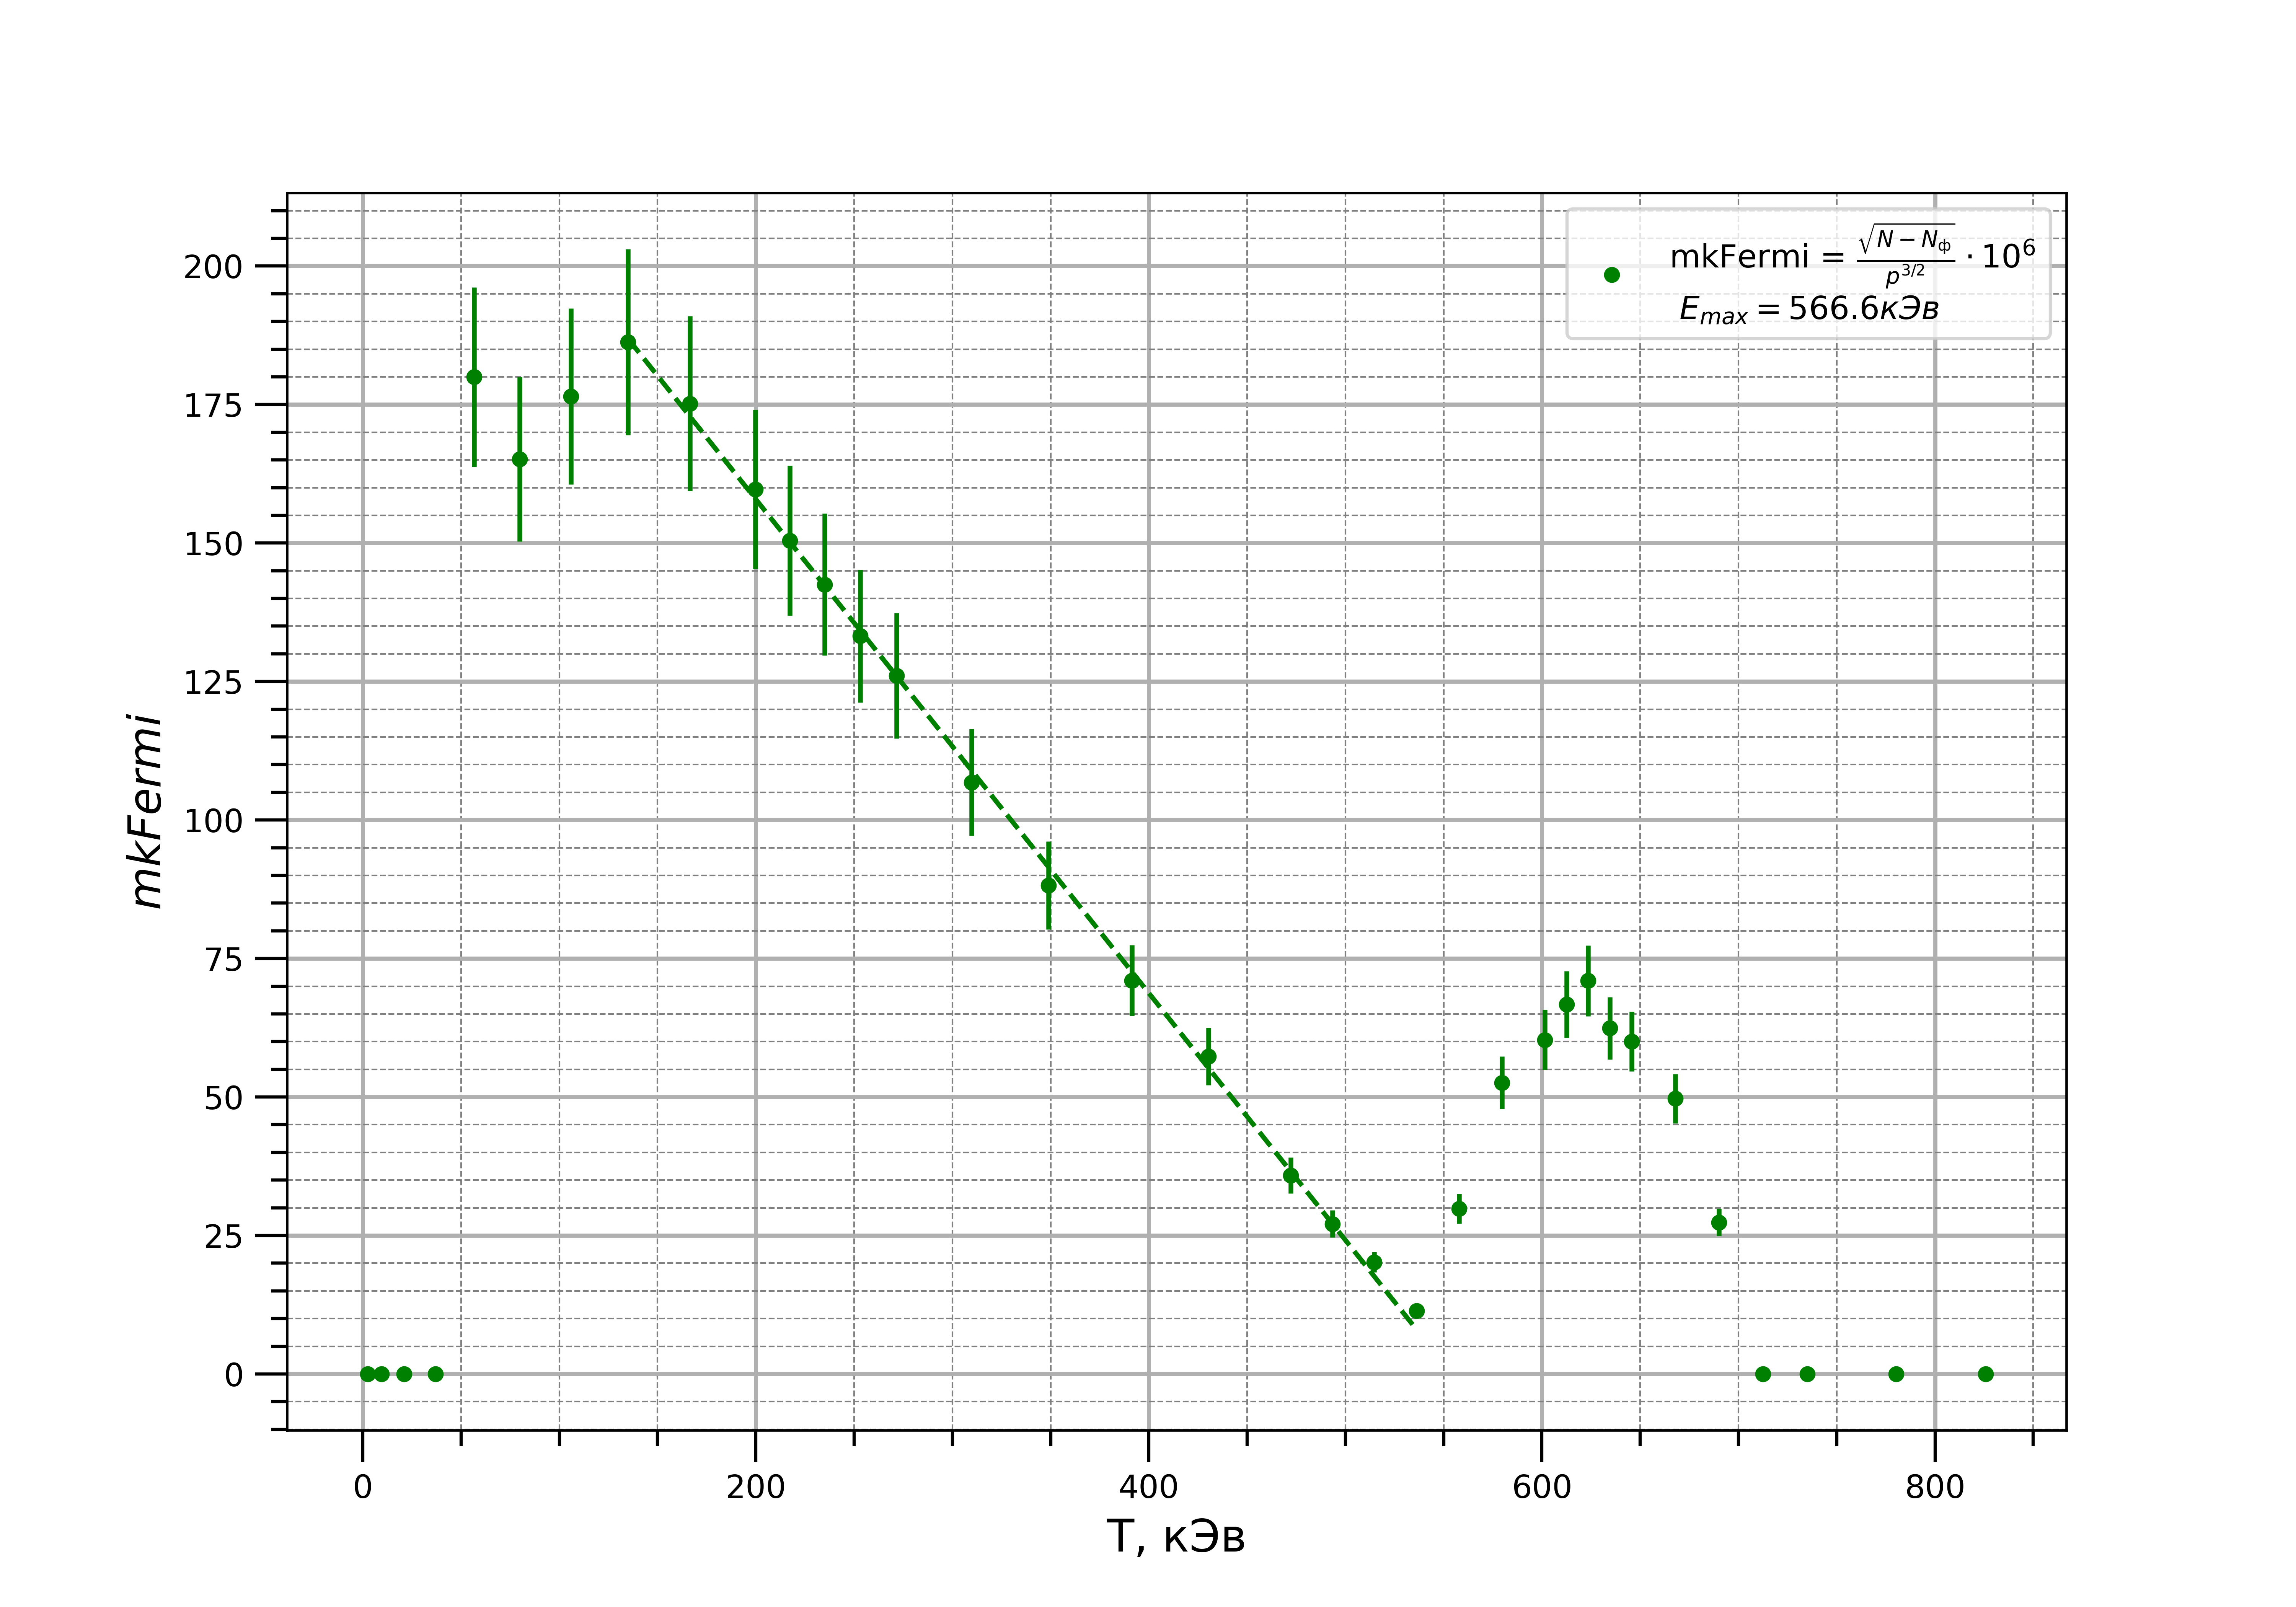
\includegraphics[scale=0.8]{mkF(T)}
			\centering
			\caption{График зависимости $\sqrt{(N(p) - \overline{N_{\text{фон}}})}/p^{3/2} \cdot 10^6) (T)$}
		\end{figure}
		
		\item  По графику Ферми-Кюри определим максимальную энергию $\beta$-спектра. Для этого проведем прямую по линейной части графика и определим точку пересечения прямой с осью абсцисс.\\
		
		\textbf{Обсуждение результатов и выводы: }\\  
		
		В ходе данной работы мы с помощью магнитного спектрометра исследовали энергетический спектр $\beta$-частиц при распаде ядер ${}^137Cs$ и определили их максимальную энергию.
		
		
		
		
		
		
		
		
		
		
		
		
		
		
		
		
		
	\end{enumerate}
	
	
	
	
	
	
	
	
	
	
	
	
	
	
	
	
	
	
	
	
	
	
	
	
	
	
	
	
	
	
	
	
	
	
	
	
	
	\end{document}